
\section{Introduction}

Simply using a formal notation does not ensure that specifications
will be correct: writing a correct formal specification is no easier
than writing a correct program or a correct description in English.
Specifications---especially {\em requirements} specifications, where
there is no higher-level specification against which they can be
verified---need to be {\em validated\/} against informal
expectations.   This is generally done by human review and inspection
(which can be very formalized processes), but with formal
specifications it is possible to do more.

The distinctive feature of {\em formal\/} specifications is that they
support formal deduction: it is possible to reduce certain questions
about a formal specification to a process that resembles calculation
and that can be checked by others or by machine.
Thus, reviews and inspections can be supplemented by {\em analyses\/}
of formal specifications, and those analyses can be mechanically checked.

In order to conduct mechanized analysis, it is necessary to support a
specification language with powerful tools including, primarily, a
theorem prover.  The needs of efficient theorem proving drive
specification language design in slightly different directions than
for unmechanized notations such as Z, but the presence of
mechanization also creates new linguistic opportunities---such as allowing
typechecking to use theorem proving---that can enhance the clarity and
precision of specifications.

PVS is a {\em verification system\/}: a specification language
tightly integrated with a powerful theorem prover and other tools.
This document is intended to serve as a first introduction to PVS: it
is not intended to teach the details of the PVS language and theorem
prover, but rather to give an appreciation of the opportunities
created by mechanized analysis in general, and of some of the
capabilities of PVS in particular.

\section{An Electronic Phone Book: Simple Version}
\markright{Phone Book: Simple Version}

Suppose we are to formally specify the requirements for an electronic phone
book, given the following informal description.\footnote{This example
is based on one by Ricky Butler and Sally Johnson of NASA
Langley~\cite{Butler&Johnson93}.}
\begin{itemize}
\item A phone book shall store the phone numbers of a city
\item It shall be possible to retrieve a phone number given a name
\item It shall be possible to add and delete entries from a phone book
\end{itemize}

Examining this description, we see that there are three types of
entities mentioned: {\em phone books}, {\em phone numbers} and {\em
names\/}; a phone book provides an association between names and
phone numbers.  We need three operations, which we can call {\em
FindPhone\/}, {\em AddPhone}, and {\em DelPhone\/}.  {\em FindPhone\/}
should take a phone book and a name and return the phone number
associated with that name.  The exact functionality of the other two
operations is less clear, so we have to make some design decisions.
We decide that {\em AddPhone} should take a phone book, a name, and a
phone number and should add the association between the name and
number to the phone book; and that {\em DelPhone\/} should take a
phone book and a name and delete the phone number associated with that
name (if any).

The next step is to decide how to represent these entities and operations
in PVS\@.  If we were programming, we would have to choose some specific
representations for phone numbers and names---e.g., ascii strings, or
more structured representations such as records containing the
area-code and number---and would have to make several design decisions
at this point.  But for requirements specification, all we require is
that phone numbers and names are distinguishable {\em types\/} of
entities.  In PVS, we can specify this as follows (a \% sign
introduces a comment that extends to the end of the line).
\begin{pvsexample}
N: TYPE              % names
P: TYPE              % phone numbers
\end{pvsexample}
These types are {\em uninterpreted\/}, meaning that we know nothing
about their members---not even whether they are zero, many, or
infinite in number---except that elements of type {\tt N} are
distinguishable from those of type {\tt P}, and that there is an
equality predicate on each type (i.e., given two {\tt P}s, it is
possible to tell whether they are the same or not).

Next, we need to describe how phone books---associations between names
and numbers---are to be represented.  There are several possibilities:
one is to record each association as a {\tt (name, phone number)}
pair, so that a phone book is a set of such pairs; another is as a
function from names to phone numbers (you can think of a function as
an array if that notion is more familiar to you).  PVS is able to
reason very effectively with functions, so there is some advantage to
the latter representation.  We can specify this as follows.
\begin{pvsexample}
B: TYPE = [N -> P]   % phone books
\end{pvsexample}
This says that phone books have the {\em type\/} {\tt
B}, and are functions from names to phone numbers.

We must recognize that not all names will be in every phone book---a
phone book only records those names that have a phone number---so we
need some way to distinguish those names that have a phone number from
those that do not.  In the specification language Z, for example, this
would be accomplished by specifying that phone books are {\em
partial\/} functions.  Efficient theorem proving, however, strongly
encourages use of {\em total\/} functions, so PVS is a logic of total
functions.\footnote{PVS can represent partial functions very nicely
using {\em dependent\/} types, but that is an advanced topic.}  One
way to indicate that a name has no phone number is to identify some
particular phone number, represented by {\tt n0} say, to indicate this
fact.  Of course we need to mentally make note that this number must
be different from any ``real'' phone number (we will see later how we
can enforce this requirement, and later still we will see a better way
to deal with this whole issue of names that have no phone number).  Given
this decision, we can next
specify the empty phone book as the (unique) phone book that maps all
names to {\tt n0}.  I will specify this axiomatically, later we will
see how to do it definitionally.
\begin{pvsexample}
n0: P
emptybook: B
emptyax: AXIOM   FORALL (nm: N): emptybook(nm) = n0
\end{pvsexample}
If we were programming an implementation, a literal translation of
this representation would be grossly inefficient: it requires
``space'' for every possible name and it explicitly records for every
name that there is no number associated with the name.  When
programming, we would seek more compact representations that traded
off space for efficient access---perhaps a hash table or balanced
binary tree.   In requirements specification, however, the idea is
simply to record the functionality required, and it is not our concern
to suggest an efficient implementation.

We can specify the {\tt FindPhone} operation as a function that takes a
phone book and a name and returns the phone number associated with
that name.
\begin{pvsexample}
FindPhone: [B, N -> P]
Findax: AXIOM   FORALL (bk: B), (nm: N):  FindPhone(bk, nm) = bk(nm)
\end{pvsexample}
Notice that this is a {\em functional\/} specification style: the
``state'' of the system we are interested in (i.e., the phone book) is
passed to the {\tt FindPhone} function as an argument; this is in contrast
to a more procedural style of specification (as in Z, for example),
where there is a built-in notion of state.  Functional specifications
use conventional logic and can be mechanized straightforwardly,
whereas procedural specifications involve some kind of Hoare
logic---for which it is rather more difficult to provide mechanized
deduction.

The distinction between functional and procedural kinds of
specification is revealed more clearly in the case of our next
operation, {\tt AddPhone.}  In a procedural specification, this operation
would update the state of the phone book ``in place.''  In the
functional style used here, we model the operation by a function that
takes a phone book, a name, and a number, and gives us back a ``new''
phone book in which the association between the name and number has
been added.   
\begin{pvsexample}
AddPhone: [B, N, P -> B]
Addax: AXIOM   FORALL (bk: B), (nm: N), (pn: P): 
   AddPhone(bk, nm, pn) = bk WITH [(nm) := pn]
\end{pvsexample}
The {\tt WITH} construct is similar to function overriding in Z.

Now that we have specified two operations, perhaps we should check our
understanding of them.  If we were programming, we might run a couple
of test cases.  Some people advocate something similar (often called
``animation'') for specifications.  This is generally feasible only
with specifications that have a constructive character (i.e., that are
essentially very high-level programs).  Not all specifications are
best presented in this way, however, so the desire to make
specifications executable can distort their other characteristics.
Another way to probe a specification is by means of ``formal
challenges.''  These are putative theorems: general statements that we
think should to be true if our specification says what it ought to.
This can yield more information than an individual test case (it is
generally equivalent to running a whole class of test cases), and uses
theorem proving (i.e., search), rather than direct execution, so it is
possible even when the specification is not constructive.  (If the
specification is constructive---as in this example---then theorem
proving generally comes down to symbolic execution and is
very efficient.)  A suitable challenge for the specification
we have so far is: ``if I add a name {\tt nm} with phone number {\tt
pn} to a phone book and look up the name {\tt nm}, I should get back
the phone number {\tt pn}.''  We can write this as follows.
\begin{pvsexample}
FindAdd: CONJECTURE  FORALL (bk: B), (nm: N), (pn: P):
  FindPhone(AddPhone(bk, nm, pn), nm) = pn
\end{pvsexample}

In order to test this conjecture, we have to extend the specification into a
complete PVS ``theory'' (as modules are called in PVS).  This is shown
in Figure~\ref{fig1}.  Then we load the specification into PVS, parse
and typecheck it, and start the prover.  The mechanics of doing this
are described in other PVS tutorial documents.  Briefly, PVS uses an
extended GNU Emacs as its interface, and PVS system functions are
invoked by Emacs keystrokes.  To invoke the prover, for example, place
the cursor on the {\tt CONJECTURE} and type {\tt M-x prove} (this will
automatically parse and typecheck if necessary).

\begin{figure}[htbp]
\begin{pvsexample}
phone_1: THEORY
BEGIN

  N: TYPE              % names
  P: TYPE              % phone numbers
  B: TYPE = [N -> P]   % phone books

  n0: P
  emptybook: B
  emptyax: AXIOM   FORALL (nm: N): emptybook(nm) = n0

  FindPhone: [B, N -> P]
  Findax: AXIOM   FORALL (bk: B), (nm: N):  FindPhone(bk, nm) = bk(nm)

  AddPhone: [B, N, P -> B]
  Addax: AXIOM   FORALL (bk: B), (nm: N), (pn: P): 
     AddPhone(bk, nm, pn) = bk WITH [(nm) := pn]

  FindAdd: CONJECTURE  FORALL (bk: B), (nm: N), (pn: P):
    FindPhone(AddPhone(bk, nm, pn), nm) = pn

END phone_1
\end{pvsexample}
\caption{\label{fig1}Specification Ready for Checking the First Challenge}
\end{figure}

%\newpage
Starting the prover on the {\tt FindAdd} conjecture produces the following
display.
\begin{pvsexample}
FindAdd :  

  |-------
{1}   FORALL (bk: B), (nm: N), (pn: P): 
        FindPhone(AddPhone(bk, nm, pn), nm) = pn

Rule? 
\end{pvsexample}
This is a \emph{sequent}: in general there will be several numbered
formulas above the turnstile symbol \verb!|-------!, and several below.
The idea is that we have to establish that the conjunction (and) of the
formulas above the turnstile implies the disjunction (or) of the
formulas below the line.  The {\tt Rule?} prompt indicates that PVS is
waiting for us to type a prover command.  These use lisp syntax, with
pieces of PVS syntax embedded in quotes: for example:
\mbox{\tt (grind :theories ("phone\_1"))}.

This introduction is intended to describe the purpose and value of
mechanized theorem proving in analysis of requirements specification;
it is not intended as a tutorial on the PVS prover, so I will not
explain all the various choices and considerations at each step.  The
prover provides a number (about 20) basic commands, and a
similar-sized collection of higher-level commands called
``strategies'' that are programmed using the basic commands.  You type
a command at the {\tt Ready?} prompt, and the prover applies the
command and presents you with the transformed sequent and another
prompt.  When the prover recognizes that a sequent is trivially true,
it terminates that branch of the proof.  Some commands may split the
proof into branches, in which case you will be presented with one of
the branches, and the others will be remembered and popped up when the
current branch terminates.  When all branches are terminated the
theorem is proved.

On straightforward theorems (and the straightforward parts of
difficult theorems), it is generally best to use the highest-level,
most automated strategies, and only to resort to the basic commands
for crucial steps.  The highest-level strategy is called {\tt grind}.
It does skolemization, heuristic instantiation, propositional
simplification (using BDDs), if-lifting, rewriting, and applies
decision procedures for linear arithmetic and equality.  It takes
several optional arguments which mostly supply the names of the
formulas that can be used for automatic rewriting (i.e., replacing of
an instance of the left hand side of an equation by the corresponding
instance of the right hand side).  In this case, we need to tell it
that all the definitions and axioms in the theory {\tt phone\_1} may
be used as rewrites.  The command above does this, and is sufficient
to prove the challenge.
\begin{pvsexample}
Rule? (grind :theories ("phone_1"))
Addax rewrites AddPhone(bk, nm, pn)
  to bk WITH [(nm) := pn]
Findax rewrites FindPhone(bk WITH [(nm) := pn], nm)
  to pn
Trying repeated skolemization, instantiation, and if-lifting,
Q.E.D.
\end{pvsexample}

Encouraged by this small confirmation that we are on the right track
we can return to specifying the {\tt DelPhone} operation.  This is
specified in a similar way to {\tt AddPhone}.
\begin{pvsexample}
DelPhone: [B, N -> B]
Delax: AXIOM   FORALL (bk: B), (nm: N): DelPhone(bk, nm) = bk WITH [(nm) := n0]
\end{pvsexample}
We can similarly test our understanding of this specification by
checking the intuition that adding a name and phone number to a book
and then deleting them leaves the book unchanged.
\begin{pvsexample}
DelAdd: CONJECTURE  FORALL (bk: B), (nm: N), (pn: P):
  DelPhone(AddPhone(bk, nm, pn), nm) = bk
\end{pvsexample}
The same proof strategy as before fails to prove the conjecture and
produces the following result.
\begin{pvsexample}
DelAdd :  

  |-------
{1}   FORALL (bk: B), (nm: N), (pn: P): DelPhone(AddPhone(bk, nm, pn), nm) = bk

Rule? (grind :theories ("phone_1"))
Addax rewrites AddPhone(bk, nm, pn)
  to bk WITH [(nm) := pn]
Delax rewrites DelPhone(bk WITH [(nm) := pn], nm)
  to bk WITH [(nm) := pn] WITH [(nm) := n0]
Trying repeated skolemization, instantiation, and if-lifting, this simplifies to: 
DelAdd :  

  |-------
{1}   bk!1 WITH [(nm!1) := pn!1] WITH [(nm!1) := n0] = bk!1

Rule?
\end{pvsexample}
The identifiers with {\tt !} in them are Skolem constants---arbitrary
representatives for quantified variables.  This sequent is requiring
us to prove that two functions (i.e., phone books) are the same: one
that has been modified by adding a name and then removing it, another
that is unchanged.  To prove that two functions are the same, we
appeal to the principle of {\em extensionality\/}, which says that
this is so if the values of the two functions are identical for every
point in their domains.
\begin{pvsexample}
Rule? (apply-extensionality)
  Applying extensionality, this simplifies to: 
DelAdd :  

  |-------
{1}   bk!1 WITH [(nm!1) := pn!1] WITH [(nm!1) := n0](x!1) = bk!1(x!1)
[2]   bk!1 WITH [(nm!1) := pn!1] WITH [(nm!1) := n0] = bk!1

Rule? (delete 2)
  Deleting some formulas, this simplifies to: 
DelAdd :  

  |-------
[1]   bk!1 WITH [(nm!1) := pn!1] WITH [(nm!1) := n0](x!1) = bk!1(x!1)

Rule? 
\end{pvsexample}
It is always possible to delete formulas from a sequent; here I have
deleted the original formula to reduce clutter, since it is the
extensional form that is interesting.  This sequent is asking us to
show that the phone number associated with an arbitrary name {\tt x!1}
is the same both before and after the phone book has been updated for
name {\tt nm!1}.  A case-analysis is appropriate here, according to
whether or not {\tt x!1 = nm!1}.  This can be accomplished by
the {\tt (lift-if)} command, which converts {\tt WITH} expressions to
their corresponding {\tt IF-THEN-ELSE} form.  The {\tt (ground)}
command (a slightly less muscular command than {\tt (grind)}) then
takes care of the various cases, except for one.
\begin{pvsexample}
DelAdd :  

  |-------
[1]   bk!1 WITH [(nm!1) := pn!1] WITH [(nm!1) := n0](x!1) = bk!1(x!1)

Rule? (lift-if)
Lifting IF-conditions to the top level,
this simplifies to: 
DelAdd :  

  |-------
{1}   IF nm!1 = x!1 THEN n0 = bk!1(x!1)
      ELSE IF nm!1 = x!1 THEN n0 = bk!1(x!1)
        ELSE bk!1(x!1) = bk!1(x!1)
        ENDIF
      ENDIF

Rule? (ground)
Applying propositional simplification and decision procedures,
this simplifies to: 
DelAdd :  

{-1}   nm!1 = x!1
  |-------
{1}   n0 = bk!1(x!1)

Rule?
\end{pvsexample}
(A {\tt (grind)} command would have performed both these steps.)
For this sequent to be true, we need to to demonstrate
that if {\tt x!1 = nm!1}, then the phone number originally associated
with {\tt x!1} is the special number {\tt n0}.  But, by virtue of the
equality, this is the same as asking us to prove that the phone number
originally associated with {\tt nm!1} is {\tt n0}---and there is no
reason why this should be true!  Suddenly, we understand the problem:
if the number associated with {\tt nm!1} beforehand was a real phone
number, {\tt nm!2}, say, then the {\tt AddPhone} operation {\em
changes\/} the association to the new number, and the {\tt DelPhone}
operation changes it again to {\tt n0}---which is not equal to {\tt
nm!2}.  Thus our conjecture is only true under the assumption that the
name we add to the phone book currently has no number associated with it.
We can test this by modifying the conjecture as follows.
\begin{pvsexample}
DelAdd2: CONJECTURE  FORALL (bk: B), (nm: N), (pn: P):
  FindPhone(bk, nm) = n0 => DelPhone(AddPhone(bk, nm, pn), nm) = bk
\end{pvsexample}
And the {\tt (grind :theories ("phone\_1"))} strategy proves this.

Another conjecture is that the result of adding a name and then
deleting it is the same as just deleting it.
\begin{pvsexample}
DelAdd3: CONJECTURE  FORALL (bk: B), (nm: N), (pn: P):
  DelPhone(AddPhone(bk, nm, pn), nm) = DelPhone(bk, nm)
\end{pvsexample}
The {\tt (grind :theories ("phone\_1"))} strategy proves this
conjecture also.

Notice how our inability to prove the original {\tt DelAdd} conjecture
exposed a deficiency in our specification and led us to discover the
source of the deficiency.  Individual test cases might have missed the
particular circumstance that exposes the problem, but the strict
requirements of mechanically checked proof systematically led us to
examine all the cases until we discovered the one that manifested the
problem.

Another conjecture we might try to prove is that after adding a name
and phone number to the phone book, the number stored for that name is
a ``real'' number (i.e., not {\tt n0}).
\begin{pvsexample}
KnownAdd: CONJECTURE  FORALL (bk: B), (nm: N), (pn: P):
  FindPhone(AddPhone(bk, nm, pn), nm) /= n0
\end{pvsexample}
The same kind of exploration with the prover will rapidly show that
this is unprovable because there is nothing that requires the {\tt
pn} argument to {\tt AddPhone} to be a ``real'' phone number.

Our exploration of this specification has revealed a couple of
deficiencies.
\begin{enumerate}
\item {\tt AddPhone} has the side effect of changing the phone number
when applied to someone who already has a number.

\item Our specification does not rule out the possibility
      of giving someone {\tt n0} as a phone number
\end{enumerate}

We can deal with the second deficiency by introducing a type {\tt GP}
of ``good phone numbers'' as a {\em subtype\/} of P, with the
constraint that {\tt n0} is not a member of {\tt GP}.  In PVS, this is
done by means of a {\em predicate subtype}, which can be written as
follows.
\begin{pvsexample}
GP: TYPE = { pn: P | pn /= n0 }
\end{pvsexample}
We will see later that predicate subtypes are a very powerful element
of the PVS specification language.  Here we can make simple use of
them by changing the {\em signature\/} of the {\tt AddPhone}
function from {\tt [B, N, P -> B]} to {\tt [B, N, GP -> B]}, and this
will automatically prevent the addition of {\tt n0} to a phone book as
a real number.

We can deal with the first deficiency noted above by dividing the
functionality of {\tt AddPhone} in two: the revised {\tt AddPhone}
will make no change to the phone book if the name concerned already
has a phone number, and the new {\tt ChangePhone} operator will change
an existing number, but will not add a number to a name that
currently lacks one.

In order to specify these functions, it is convenient to add a
predicate {\tt Known?} that takes a phone book and a name and returns
{\tt true} if that name has a ``real'' phone number in the book
concerned.  (A {\em predicate\/} is just a function whose range type
is boolean.)  This can be specified as follows.
\begin{pvsexample}
Known?: [B, N -> bool]
Known_ax: AXIOM FORALL (bk: B), (nm: N): Known?(bk, nm) = (bk(nm) /= n0)
\end{pvsexample}

This axiomatic style of specification has the disadvantage that axioms
can introduce inconsistencies.  An individual axiom is seldom
dangerous: rather, danger lies in the interactions among several
axioms.  For example, with the original signature and definition of
{\tt AddPhone}, adding the following axiom to that above yields an
inconsistent specification.
\begin{pvsexample}
Whoops: AXIOM   FORALL (bk: B), (nm: N), (pn, P): Known?(AddPhone(bk, nm, pn), nm)
\end{pvsexample}

Inconsistent specifications are dangerous because they can be used to
prove anything at all,\footnote{For example, when used in conjunction
with the {\tt AXIOM}s {\tt emptyax}, {\tt Known\_ax}, and {\tt Addax},
{\tt Whoops} allows us to prove {\tt true = false}.}
and because they cannot be implemented.  It is
disturbingly easy to introduce inconsistent axioms, so it is generally
best to use them sparingly.  Axioms are really needed only when it is
necessary to constrain (rather than fully define) the values of a
function, or when it is necessary to constrain the interactions of
several functions.  When the intent is to fully define the values of
a function, it is generally better to state it as a {\em definition\/},
since PVS will then check that it is indeed a ``conservative
extension'' (and therefore does not introduce an inconsistency).

The predicate {\tt Known?} can be introduced by means of a definition
by replacing the two lines used earlier (the specification of its
signature and axiom) by the following single line.
\begin{pvsexample}
Known?: [B, N -> bool] = LAMBDA (bk: B), (nm: N): bk(nm) /= n0
\end{pvsexample}
The use of {\tt LAMBDA} notation can be a little daunting, so PVS allows an
alternative, ``applicative,'' form of definition as follows.
\begin{pvsexample}
Known?(bk: B, nm: N): bool = bk(nm) /= n0
\end{pvsexample}
The need to specify the types of the variables in this declaration
can be eliminated by declaring them separately.
\begin{pvsexample}
bk: VAR B
nm: VAR N
Known?(bk, nm): bool = bk(nm) /= n0
\end{pvsexample}
In this way, the previous axiomatic specification for {\tt AddPhone} can be
changed to the following definition, which incorporates the refinement
that the function does not change the phone book if the name already
has a number known for it.
\begin{pvsexample}
gp: VAR GP
AddPhone(bk, nm, gp): B = 
  IF Known?(bk, nm) THEN bk ELSE bk WITH [(nm) := gp] ENDIF
\end{pvsexample}
We can check that these changes provide some of the properties we
expect by considering the following formal challenge.
\begin{pvsexample}
KnownAdd: CONJECTURE  FORALL bk, nm, gp: Known?(AddPhone(bk, nm, gp), nm)
\end{pvsexample}
This says that a name is definitely known (i.e., has a ``real'' phone
number) after applying {\tt AddPhone} to it.   Notice that since the
variables {\tt bk}, {\tt nm}, and {\tt gp} have already been declared,
there is no need to specify their types in the {\tt FORALL} construction.
In fact, there is no need to provide the {\tt FORALL} construction at all:
the following specification is equivalent to the one above, since PVS
automatically interprets ``free'' variables as universally quantified
at the outermost level.
\begin{pvsexample}
KnownAdd: CONJECTURE  Known?(AddPhone(bk, nm, gp), nm)
\end{pvsexample}
This conjecture is easily proved by the {\tt grind} strategy.

\begin{figure}[htbp]
\begin{pvsexample}
phone_2: THEORY

BEGIN

  N: TYPE              \% names
  P: TYPE              \% phone numbers
  B: TYPE = [N -> P]   \% phone books

  n0: P

  GP: TYPE = {pn: P | pn /= n0}

  nm: VAR N
  pn: VAR P
  bk: VAR B
  gp, gp1, gp2: VAR GP

  emptybook(nm): P = n0

  FindPhone(bk, nm): P = bk(nm)

  Known?(bk, nm): bool = bk(nm) /= n0

  AddPhone(bk, nm, gp): B = 
    IF Known?(bk, nm) THEN bk ELSE bk WITH [(nm) := gp] ENDIF

  ChangePhone(bk, nm, gp): B = 
    IF Known?(bk, nm) THEN bk WITH [(nm) := gp] ELSE bk ENDIF

  DelPhone(bk, nm): B = bk WITH [(nm) := n0]

  FindAdd: CONJECTURE
    NOT Known?(bk, nm) => FindPhone(AddPhone(bk, nm, gp), nm) = gp

  FindChange: CONJECTURE
    Known?(bk, nm) => FindPhone(ChangePhone(bk, nm, gp), nm) = gp

  DelAdd: CONJECTURE
    DelPhone(AddPhone(bk, nm, gp), nm) = DelPhone (bk, nm)

  KnownAdd: CONJECTURE Known?(AddPhone(bk, nm, gp), nm)

  AddChange: CONJECTURE
    ChangePhone(AddPhone(bk, nm, gp1), nm, gp2) =
      AddPhone(ChangePhone(bk, nm, gp2), nm, gp2)

END phone_2
\end{pvsexample}
\caption{\label{fig2}Revised Specification}
\end{figure}
Proceeding in this way, we can construct the theory {\tt phone\_2}
shown in Figure~\ref{fig2}.  All the conjectures in that theory
are proved by the simple command {\tt (grind)}.   There is no need to
specify auto-rewriting of the {\tt phone\_2} theory, since definitions
are automatically available for rewriting (another advantage that they
have over axioms).

If we try to add the dangerous {\tt AXIOM} {\tt Whoops} to this new
specification, PVS will note that the third argument supplied to {\tt
Addphone} {\tt (pn}) is a {\tt P}, whereas the signature of {\tt
AddPhone} says it requires a {\tt GP} in this position.  PVS allows a
value of a supertype to be used where one of a subtype is required,
provided the value can be proven, in its context, to satisfy the
predicate of the subtype concerned.  The corresponding proof
obligation is generated automatically by PVS as a Type-Correctness
Condition (TCC).  PVS does not consider a specification fully
typechecked until all its TCCs have been proved (though you can
postpone doing the proof until convenient).  TCCs are displayed by the
command {\tt M-x show-tccs}; in the present case, the TCC generated by
{\rm Whoops} is the following.
\begin{pvsexample}
% Subtype TCC generated (line 37) for pn
  % untried
whoops_TCC1: OBLIGATION (FORALL (pn: P): pn /= n0);
\end{pvsexample}
This is obviously unproveable (and untrue!), and the folly of adding
the axiom {\tt Whoops} is thereby brought to our attention.

Notice that if the {\tt pn} in {\tt Whoops} is changed to {\tt gp},
then the formula not only becomes harmless (and no TCC is generated),
but a proveable consequence of the definitions.

\newpage
\markright{Phone Book: Better Version}
\section{A Better Version of the Specification Using Sets}
\markright{Phone Book: Better Version}

The realization that {\tt AddPhone} had the effect of changing the
phone number associated with a name if that name already had a phone
number led us to revise the specification so that {\tt AddPhone} has
no effect when the name already has a phone number.  This treatment
assumes that names can have at most one phone number associated with
them.  On reflection, or after consultation with the customer, we may
decide that it is better to allow names to
have multiple numbers associated with them.  We can accommodate this
by changing the range of the phone book function from a single phone
number to a {\em set\/} of phone numbers as follows.
\begin{pvsexample}
B: TYPE = [N -> setof[P]]   \% phone books
\end{pvsexample}
This approach has the benefit that we now have a ``natural''
representation for names that do not have phone numbers: they can be
associated with the emptyset of phone numbers.

A specification based on this approach is shown in Figure~\ref{fig3}.
The set-constructing functions such as {\tt add}, {\tt remove}, {\tt
emptyset}, etc., and the predicates on sets such as {\tt disjoint?}
are defined in a PVS {\em prelude\/} (i.e., built-in)
theory called {\tt set}.  You can inspect this theory with the command
{\tt M-x view-prelude-theory}.
\begin{figure}[htbp]
\begin{pvsexample}
phone_3 : THEORY

  BEGIN

  N: TYPE                     % names
  P: TYPE                     % phone numbers
  B: TYPE = [N -> setof[P]]   % phone books
  nm, x: VAR N
  pn: VAR P
  bk: VAR B
  
  emptybook(nm): setof[P] = emptyset[P]

  FindPhone(bk, nm): setof[P] = bk(nm)

  AddPhone(bk, nm, pn): B = bk WITH [(nm) := add(pn, bk(nm))]

  DelPhone(bk,nm): B = bk WITH [(nm) := emptyset[P]]

  DelPhoneNum(bk,nm,pn): B = bk WITH [(nm) := remove(pn, bk(nm))]

  FindAdd: CONJECTURE member(pn, FindPhone(AddPhone(bk, nm, pn), nm))

  DelAdd: CONJECTURE DelPhoneNum(AddPhone(bk, nm, pn), nm, pn) =
                DelPhoneNum(bk, nm, pn)

  END phone_3
\end{pvsexample}
\caption{\label{fig3}Specification Using Set Constructions}
\end{figure}
A rather more attractive rendition of this specification is shown in
Figure~\ref{fig3-latex}; this is produced by the command {\tt M-x
latex-theory}, which typesets the specification using \LaTeX.

\begin{figure}
\def\pvsdeclspacing{-2mm}
\input{phone_3}
\caption{\label{fig3-latex}\LaTeX-Printed Version of the Specification
in Figure~\protect\ref{fig3}}
\end{figure}
The first conjecture in this specification is easily proved using {\tt
(grind)}.   The second one requires the more complex proof shown
below.
\begin{pvsexample}
("" (GRIND)
    (APPLY-EXTENSIONALITY)
    (DELETE 2)
    (LIFT-IF)
    (GROUND)
    (APPLY-EXTENSIONALITY)
    (DELETE 2)
    (GRIND))
\end{pvsexample}
This is the form in which PVS proofs are stored for later replay.

We have specified single additions to the phone book, but it seems
likely that bulk additions will also be necessary.  This will give us
an opportunity to explore some more advanced features of the PVS
language and prover.  We would like to specify a function {\tt
AddList}, say, that takes a phone book and some collection of names
and phone numbers and adds all of those names and phone numbers to the
phone book.  Each name-and-number is a pair, which can be represented
in PVS by the tuple-type {\tt [N, P]}.  We could represent a
collection of such pairs by either a sequence, or a list---a list is
most convenient here, and is represented in PVS by the type {\tt
list[[N, P]]}.  In this expression, the outermost brackets enclose the
type parameter (here {\tt [N, P]}) to the generic {\tt list} theory
(e.g., a list of phone numbers would be {\tt list[P]}).  In order to
process such a list, we specify {\tt AddList} as a recursive function
that returns the phone book it is given if the list is empty, and
otherwise recurses by applying the tail of the list to the phone book
that results from applying {\tt AddPhone} to the first name and number
pair in the list.

\begin{pvsexample}
updates: VAR list[[N, P]]

AddList(bk, updates): RECURSIVE B = 
  CASES updates OF
    null: bk,
    cons(upd, rest): AddList(AddPhone(bk, proj_1(upd), proj_2(upd)), rest)
  ENDCASES
  MEASURE length(updates)
\end{pvsexample}

In this specification, the {\tt CASES} expression introduces a
pattern-matching enumeration over the constructors of an abstract data
type (here, {\tt list}), and the {\tt proj\_i} functions project out
the {\tt i}'th member of a tuple.  The {\tt MEASURE} clause indicates
the argument that decreases across recursive calls (more generally, it
specifies a function of the arguments, and an ordering relation
according to which it decreases).  PVS uses the {\tt MEASURE} to
generate a TCC to ensure that the function is total (i.e., that the
recursion always ``terminates'').  In this case, the TCC is
\begin{pvsexample}
% Termination TCC generated (line 48) for AddList

  AddList_TCC1: OBLIGATION
      (FORALL (rest: list[[N, P]], upd: [N, P], updates: list[[N, P]]):
         updates = cons[[N, P]](upd, rest)
           IMPLIES length[[N, P]](rest) < length[[N, P]](updates))
\end{pvsexample}
and it is proved automatically by PVS's standard strategy for proving
TCCs (this strategy, called {\tt (tcc)}, is a variety of {\tt (grind)}).

The {\tt list} datatype is specified in the PVS prelude using the
datatype construction (similar to a ``free type'' in Z).
\begin{pvsexample}
list [T: TYPE]: DATATYPE 
 BEGIN
  null: null?
  cons (car: T, cdr:list):cons?
 END list
\end{pvsexample}
This specifies that {\tt list} is a datatype that takes a single type
parameter and has constructors {\tt null} and {\tt cons}, with
corresponding recognizers and predicate subtypes {\tt null?} and {\tt
cons?}, and accessors {\tt car} and {\tt cdr}.  This specification
expands internally into many axioms and definitions that are
guaranteed to be conservative (i.e., not to introduce
inconsistencies), and that are used very efficiently by the prover.

To validate our understanding of this function, we can try a couple of
challenges.  A reasonable expectation is that if a number is a member
of the set of phone numbers for a given name, then it is still a member
of that set after an arbitrary list of names and phone numbers have
been added to the phone book.
\begin{pvsexample}
AddList_member: CONJECTURE
  member(pn, FindPhone(bk, nm)) =>
     member(pn, FindPhone(AddList(bk, updates), nm))
\end{pvsexample}
Like most conjectures involving recursively-defined functions, this
one requires a proof by induction.  PVS provides some powerful
strategies for inductive proofs.  Here, the single strategy
{\tt (induct-and-simplify "updates" :defs t)}
is sufficient to prove the challenge.  The argument {\tt "updates"} is
the name of the variable on which to induct, and {\tt :defs t}
instructs PVS that it may treat all definitions as rewrites.  PVS
automatically selects the correct induction rule (here, induction on
lists), based on the type of the induction variable.  The induction
rule itself is defined automatically as part of the expansion of the
{\tt list} datatype definition.

A rather more complicated conjecture is that the set of phone numbers
associated with a given name is unchanged when a list of names and
phone numbers are added to the phone book if the given name is not
mentioned in the list.  This can be specified as follows.
\begin{pvsexample}
FindList: CONJECTURE
  (every! (upd:[N, P]): proj_1(upd)/=nm) (updates) =>
    FindPhone(AddList2(bk, updates), nm) = FindPhone(bk, nm)
\end{pvsexample}
In this specification, {\tt every!} introduces the body of a predicate
that is true of all members of the list supplied as its argument
(here, {\tt updates}).  It is another of the constructions defined
automatically as a result of expanding the {\tt list} datatype
definition.  As with the previous example, the {\tt
induct-and-simplify} strategy is able to prove this conjecture
automatically.

%\newpage

\markright{Phone Book: Version with Invariant}
\section{Version of the Specification That Maintains An Invariant}
\markright{Phone Book: Version with Invariant}


A reasonable expectation is that the same phone number is never
assigned simultaneously to two different names.  We can extend the
specification to ensure this by adding a predicate {\tt
UnusedPhoneNum} that returns {\tt true} if a given number is not
assigned to any name in a given phone book, and  then modifying
{\tt AddPhone} to check the  number being added is indeed unused.
\begin{pvsexample}
UnusedPhoneNum(bk, pn): bool =
   (FORALL nm: NOT member(pn,FindPhone(bk, nm)))

AddPhone(bk, nm, pn): B = 
  IF UnusedPhoneNum(bk, pn) THEN bk WITH [(nm) := add(pn, bk(nm))]
    ELSE bk
  ENDIF
\end{pvsexample}

If we've got this right, then it ought to be the case that the sets of
phone numbers assigned to different names are always disjoint.  We
could generate a few challenges to check this, but we really want to
be sure that the disjointness condition is an {\em invariant\/} of the
specification.  Recognizing this, we could try to generate the proof
obligations that ensure this property.   It is tedious and
error-prone to generate proof obligations of this kind by hand, so
some systems have special provision for generating the proof
obligations necessary to guarantee invariants.  PVS, however, can
generate the necessary proof obligations as part of a much more
general mechanism.

We have already seen that PVS allows predicate subtypes.  The first
step is to define those phone books that are ``valid'' as the subtype {\tt VB}
of phone books in which the sets of numbers associated with different
names are disjoint.
\begin{pvsexample}
VB: TYPE = { b:B | (FORALL (x,y: N): x /= y => disjoint?(b(x), b(y))) }
\end{pvsexample}
Then we change the specification of {\tt FindPhone} to specify that it takes
a {\tt VB} and returns a {\tt VB}:
\begin{pvsexample}
bk: VAR VB

AddPhone(bk, nm, pn): VB = 
  IF UnusedPhoneNum(bk, pn) THEN bk WITH [(nm) := add(pn, bk(nm))]
    ELSE bk
  ENDIF
\end{pvsexample}
Now the expression {\tt bk WITH [(nm) := add(pn, bk(nm))]} appearing
here is a {\tt B}, but not necessarily a {\tt VB}.  But in order to
satisfy the return type specified for {\tt AddPhone}, this expression
must be a {\tt VB}\@.  As already explained, PVS allows a value of a
supertype to be used where one of a subtype is required, provided the
value can be proven, in its context, to satisfy the predicate of the
subtype concerned.  The context here is {\tt UnusedPhoneNum(bk, pn)},
so the proof obligation that needs to be discharged in order to ensure
this specification is well-typed is the following.
\begin{pvsexample}
% Subtype TCC generated (at line 22, column 34) for
    % bk WITH [(nm) := add(pn, bk(nm))]
    % expected type  VB
  % proved - complete
AddPhone_TCC1: OBLIGATION
  FORALL (bk: VB, nm: N, pn: P):
    UnusedPhoneNum(bk, pn) IMPLIES
     (FORALL (x, y: N):
        x /= y =>
         disjoint?[P](bk WITH [(nm) := add[P](pn, bk(nm))](x),
                      bk WITH [(nm) := add[P](pn, bk(nm))](y))));
\end{pvsexample}
This proof obligation is called a Type-Correctness Condition (TCC) and
it is generated automatically by PVS\@.  
Proving it requires the following steps.
\begin{pvsexample}
("" (GRIND :IF-MATCH NIL)
    (("1" (GRIND)) ("2" (INST -1 "x!1" "y!1")
                        (GRIND))
                   ("3" (GRIND))
                   ("4" (INST -1 "x!1" "y!1")
                        (GRIND))
                   ("5" (INST -1 "x!1" "y!1")
                        (GRIND))))
\end{pvsexample}
Notice that the proof splits into several branches after the first
step.  PVS can generate a graphical display of the proof tree---which
can then be saved as a postscript file---using the command {\tt M-x
x-show-proof}.  The output for this proof is shown in
Figure~\ref{proof-pic},

\begin{figure}[htb]
\begin{center}
%\leavevmode\epsfxsize=1.0\hsize\epsfbox{phone_4_AddPhone_TCC1.ps}\mbox{}
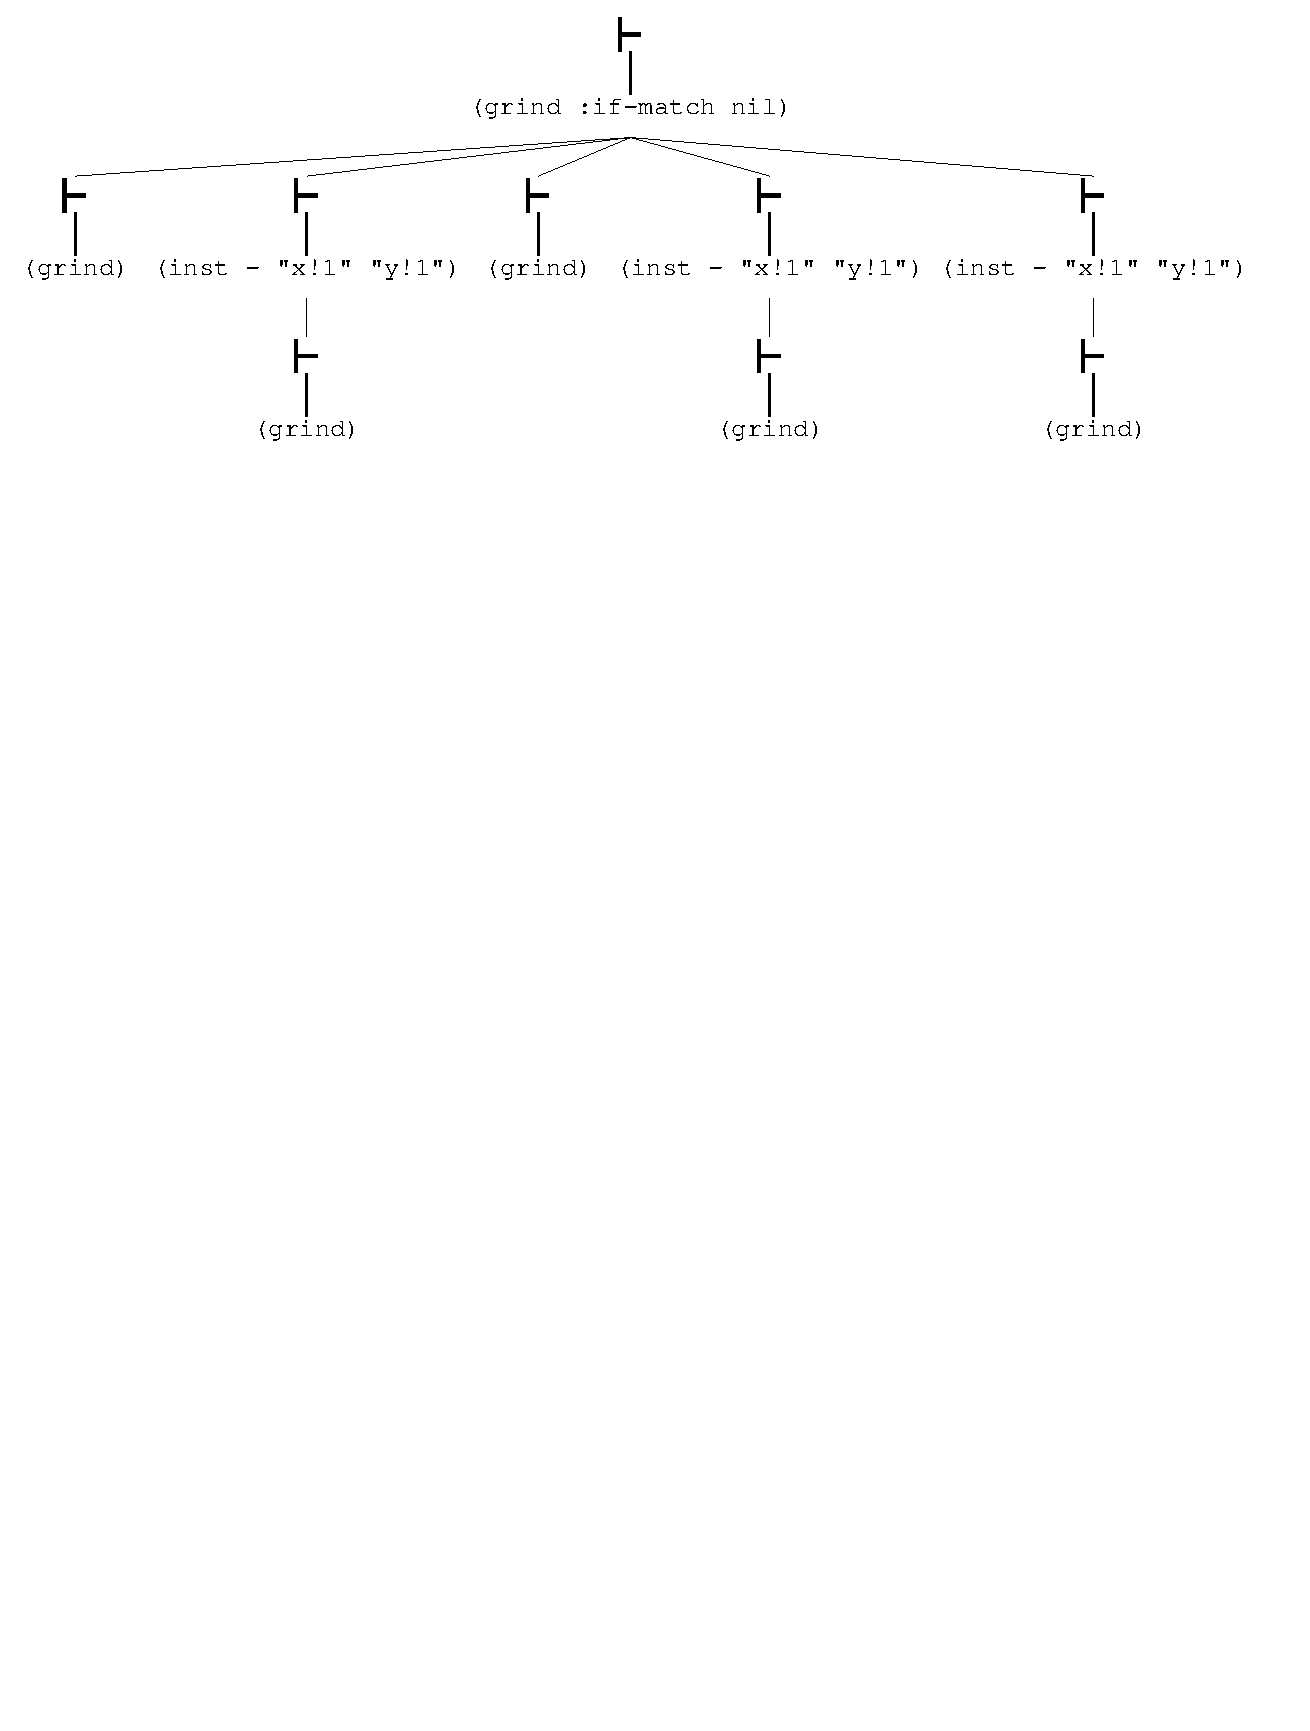
\includegraphics[width=\linewidth]{phone_4_AddPhone_TCC1}
\end{center}
\caption{\label{proof-pic}Graphical Display of the Proof Tree for
TCC {\tt AddPhone\_TCC1}}
\end{figure}

The important point to note, however, is that the close integration
between language and prover in PVS allows the mechanization of very
strong checks on specifications.

The full version of the specification of the previous section,
adjusted to ensure that only valid phone books are generated is shown
in figure~\ref{fig4} and the TCCs generated are shown in
Figure~\ref{fig4-tccs}.

\begin{figure}
\def\pvsdeclspacing{-2mm}
\input{phone_4}
\caption{\label{fig4}Specification Enforcing the Invariant that
Different Names Have Disjoint Sets of Phone Numbers}
\end{figure}

\begin{figure}
\begin{pvsexample}
% Subtype TCC generated (at line 14, column 19) for
    % (LAMBDA (x: N): emptyset[P])
    % expected type  VB
  % proved - complete
emptybook_TCC1: OBLIGATION
  FORALL (x_1, y: N): x_1 /= y => disjoint?[P](emptyset[P], emptyset[P]);

% Subtype TCC generated (at line 22, column 34) for
    % bk WITH [(nm) := add(pn, bk(nm))]
    % expected type  VB
  % proved - complete
AddPhone_TCC1: OBLIGATION
  FORALL (bk: VB, nm: N, pn: P):
    UnusedPhoneNum(bk, pn) IMPLIES
     (FORALL (x_1, y: N):
        x_1 /= y =>
         disjoint?[P]
             ((bk WITH [(nm) := add[P](pn, bk(nm))])(x_1),
              (bk WITH [(nm) := add[P](pn, bk(nm))])(y)));

% Subtype TCC generated (at line 27, column 24) for
    % bk WITH [(nm) := emptyset[P]]
    % expected type  VB
  % proved - complete
DelPhone_TCC1: OBLIGATION
  FORALL (bk: VB, nm: N):
    FORALL (x_1, y: N):
      x_1 /= y =>
       disjoint?[P]
           ((bk WITH [(nm) := emptyset[P]])(x_1),
            (bk WITH [(nm) := emptyset[P]])(y));

% Subtype TCC generated (at line 29, column 30) for
    % bk WITH [(nm) := remove(pn, bk(nm))]
    % expected type  VB
  % proved - complete
DelPhoneNum_TCC1: OBLIGATION
  FORALL (bk: VB, nm: N, pn: P):
    FORALL (x_1, y: N):
      x_1 /= y =>
       disjoint?[P]
           ((bk WITH [(nm) := remove[P](pn, bk(nm))])(x_1),
            (bk WITH [(nm) := remove[P](pn, bk(nm))])(y));
\end{pvsexample}
\caption{\label{fig4-tccs}TCCs for the Specification of Figure \protect\ref{fig4}}  
\end{figure}

\newpage

\section{Summary}

It is no easier to write correct specifications than to write correct
programs; just like programs, specifications need to be validated
against their informal requirements and expectations.  The
mechanization provided by PVS allows the human inspections and
reviews that are an essential element of validation to be
supplemented by mechanically checked analyses.

I hope the example considered here has conveyed some appreciation for
the opportunities created by mechanically supported formal
specification.  Other tutorials describe more of the mechanics of
using PVS, and give examples of its use to verify algorithm
correctness and to prove difficult theorems.


